\documentclass[acmsmall,nonacm]{acmart}

\usepackage{booktabs}
\usepackage{multirow}
\usepackage{tikz}
\usetikzlibrary{positioning,arrows.meta}

\begin{document}

\title{Native or Translate-Test? A Controlled Study of Multilingual Scientific Question Answering in Hindi and Odia}

\author{Kota Kousalanjan}
\email{mai2026015@iiita.ac.in}
\affiliation{%
  \institution{Indian Institute of Information Technology Allahabad}
  \city{Prayagraj}
  \country{India}}

\begin{abstract}
On general-domain Indic question answering, translating the input into English first (Translate-Test, TT) has been reported to beat native processing for very low-resource languages, while native processing is competitive for mid-resource ones. We test whether this holds for \emph{scientific} evidence. We run a pre-registered, paired comparison on the official 500-question PubMedQA test set, machine-translated into Hindi (mid-resource) and Odia (very low-resource) with IndicTrans2, using a zero-shot Qwen2.5-1.5B-Instruct model. Our evaluation code reproduces the published Majority baseline exactly. TT beats native input by $+12.88$ macro-F1 for Hindi (95\% CI $[+7.79, +17.87]$) and $+12.42$ for Odia ($[+7.09, +17.58]$), both with Holm-adjusted $p < 10^{-6}$, and recovers nearly all of the English score (44.59). Native input mostly fails because the model almost stops answering ``no''. The predicted TT advantage for Odia holds, but the predicted parity for Hindi does not: the two gaps do not differ detectably (difference $+0.46$, CI $[-5.01, +6.13]$). Odia also costs more tokens and loses more numbers in translation (81.5\% vs 93.5\% preserved). Because TT here is a machine-translation round trip of English text, these results describe this design and model, not native-authored documents.
\end{abstract}

\keywords{multilingual LLMs, translate-test, scientific question answering, PubMedQA, Indic languages, tokenization}

\maketitle

%% ===================================================================
\section{Introduction}

In my earlier survey of multilingual robustness in LLMs for scientific literature analysis, I argued that the Translate-Test (TT) strategy ``should be compared with native processing'' for scientific text. This paper performs that comparison.

The motivation comes from Singh et al.~\cite{singh2025indicqa}. On a general-domain Indic QA benchmark they found that TT outperforms multilingual LLMs for low-resource languages such as Odia and Punjabi, whereas native input scores better for mid-resource Hindi and Marathi. Scientific text differs from general text in ways that could change this picture. Evidence in biomedical abstracts is carried by numbers and technical terms, and translation errors are known to hit low-resource languages hardest~\cite{agrawal2024translation}. Tokenizers also charge very different prices for the same content in different languages~\cite{ahia2023tokens}.

\paragraph{Research questions.}
\textbf{RQ1:} On evidence-based biomedical yes/no/maybe QA, does TT outperform native processing, and does this depend on the language's resource tier?
\textbf{RQ2:} How consistent are a model's answers across languages, relative to its own English answers?
\textbf{RQ3:} How do token cost and number preservation through translation relate to failures?
Following~\cite{singh2025indicqa}, we hypothesised \textbf{H1}: TT $>$ native for Odia; \textbf{H2}: native $\geq$ TT for Hindi; and, following~\cite{agrawal2024translation}, \textbf{H3}: numbers are preserved less often for Odia than for Hindi.

\paragraph{Contribution.}
This is not a new method. It is a controlled test of whether a published general-domain finding transfers to scientific QA, with a pre-registered protocol, a validated evaluation pipeline, and an analysis of baseline behaviour and translation cost. Its main finding is negative for transfer: for a small model, TT helps a mid-resource language as much as a very low-resource one.

%% ===================================================================
\section{Related Work}

\textbf{Scientific QA.} PubMedQA~\cite{jin2019pubmedqa} asks whether a research question is answered yes, no or maybe by the abstract of a PubMed article. Its 1,000 expert-labelled items (PQA-L) have an official 500-item test set. Reported test results include Majority 55.20/23.71 (accuracy/macro-F1), single human 78.00/72.19, and 68.1\% accuracy for the best fine-tuned BioBERT. PubMedQA is English-only.

\textbf{Translate-Test vs native.} Singh et al.~\cite{singh2025indicqa} report the tier-dependent TT/native pattern described above on 11 Indic languages. Yeginbergen et al.~\cite{yeginbergen2026crosslingual} study multilingual medical QA and find that combining English and target-language retrieval helps low-resource languages most. Their work covers Basque and Kazakh, not Indic languages.

\textbf{Translation and tokenization.} Agrawal et al.~\cite{agrawal2024translation} show that translation inconsistencies in XNLI disproportionately affect low-resource languages, including Hindi. Ahia et al.~\cite{ahia2023tokens} document large cross-lingual differences in token cost. BenchMAX~\cite{huang2025benchmax} illustrates the effort needed to make translated benchmarks trustworthy, which is a caveat for our machine-translated inputs.

%% ===================================================================
\section{Method}

\begin{figure}[t]
\centering
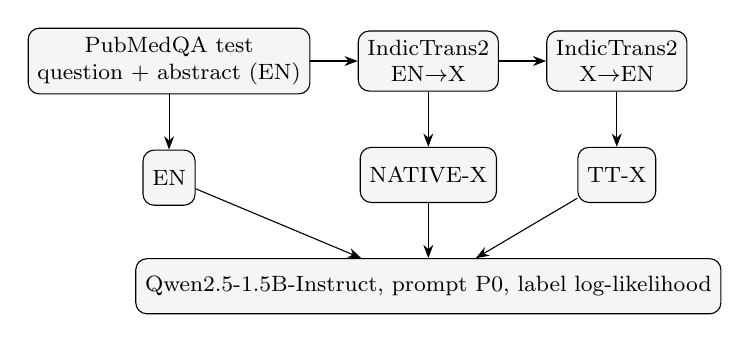
\begin{tikzpicture}[node distance=4mm and 6mm, font=\footnotesize,
  box/.style={draw, rounded corners, align=center, minimum height=7mm, fill=gray!8},
  ar/.style={-{Stealth}}]
\node[box] (src) {PubMedQA test\\question + abstract (EN)};
\node[box, right=of src] (fwd) {IndicTrans2\\EN$\to$X};
\node[box, right=of fwd] (back) {IndicTrans2\\X$\to$EN};
\node[box, below=7mm of src] (en) {EN};
\node[box, below=7mm of fwd] (nat) {NATIVE-X};
\node[box, below=7mm of back] (tt) {TT-X};
\node[box, below=7mm of nat, minimum width=55mm] (llm) {Qwen2.5-1.5B-Instruct, prompt P0, label log-likelihood};
\draw[ar] (src) -- (fwd); \draw[ar] (fwd) -- (back);
\draw[ar] (src) -- (en); \draw[ar] (fwd) -- (nat); \draw[ar] (back) -- (tt);
\draw[ar] (en) -- (llm); \draw[ar] (nat) -- (llm); \draw[ar] (tt) -- (llm);
\end{tikzpicture}
\caption{Pipeline. NATIVE and TT start from the same EN$\to$X translation (X $\in$ \{Hindi, Odia\}). They differ only in the X$\to$EN step and in the language the model reads.}
\label{fig:pipeline}
\end{figure}

\textbf{Data.} We use PQA-L from the official repository (commit \texttt{1cbae8e}, MIT licence). The official 500-item test set is used once per condition. The remaining 500 items form a development set, used only for pipeline checks and the baseline gate. Only the \texttt{QUESTION} and \texttt{CONTEXTS} fields reach the model. The fields \texttt{LONG\_ANSWER}, \texttt{reasoning\_required\_pred} and \texttt{reasoning\_free\_pred} contain the answer, and a unit test asserts that they never enter a prompt (all 1,000 items).

\textbf{Conditions} (Figure~\ref{fig:pipeline}). \emph{EN}: the original English. \emph{NATIVE-X}: question and abstract machine-translated into X. \emph{TT-X}: the NATIVE-X text translated back into English. NATIVE simulates reading a paper written in X; TT simulates translating it to English first. The instruction and answer words stay in English in every condition, so only the language of the evidence varies.

\textbf{Translation.} We use IndicTrans2 distilled 200M models~\cite{gala2023indictrans2} in both directions (beam 5, sentence-level, cached once and reused by every condition).

\textbf{Model and scoring.} We use Qwen2.5-1.5B-Instruct~\cite{qwen2025qwen25} with its chat template. For each item we compute the summed log-probability of `` yes'', `` no'' and `` maybe'' after the prefix ``Answer:'' and predict the argmax, with no sampling. All three labels are single tokens for this tokenizer.

\textbf{Metrics and statistics.} The primary metric is macro-F1, because labels are imbalanced (55.2/33.8/11.0\% yes/no/maybe). The primary contrast is $\Delta = $ macro-F1(TT) $-$ macro-F1(NATIVE) per language, with a paired bootstrap 95\% CI (10,000 resamples) and an exact McNemar test on per-item correctness, Holm-corrected over the two languages. An effect is claimed only if both criteria agree. RQ2 uses agreement and Cohen's $\kappa$ against the model's own EN predictions. RQ3 uses token fertility (full-prompt tokens under NATIVE $\div$ under EN, so the shared English instruction is included) and the share of source numbers recovered after translation, with native digits normalised.

%% ===================================================================
\section{Experimental Setup}

\textbf{Pre-registration.} The protocol is a hashed YAML file. Version 1 was frozen before any model output existed. It was revised three times, after development-split outputs but each time \emph{before any test-split output existed}, and each revision is logged with its reason. v2 moved to 1--1.5B models after 3B fp16 models did not fit the available 8\,GB machine. v3 removed a second model (Llama-3.2-1B) for compute reasons. v4 reduced the languages to one per tier (Hindi, Odia) and dropped a prompt-sensitivity analysis.

\textbf{Environment.} Development runs used Apple M1 (MPS), Python 3.13.5, PyTorch 2.9.1 and transformers 4.57.3. Translation requires transformers 4.51.3: newer versions crash IndicTrans2's remote code, which expects legacy cache tuples. Test runs use a Colab T4 GPU (fp16). The seed is 2026 throughout.

%% ===================================================================
\section{Results}

\subsection{Pipeline validation}
Our evaluation code reproduces the published Majority baseline \emph{exactly} on the official test set: 55.20 accuracy and 23.71 macro-F1, matching Table~5 of~\cite{jin2019pubmedqa}. Dev and test splits are disjoint, the test PMIDs and labels match the official ground truth, and the label distribution matches the published one.

\subsection{Baseline validation (English, dev)}

\begin{table}[t]
\caption{English zero-shot baseline on the development split (n = 500) and published reference points. Published values are on the test split and are shown only as a plausibility range.}
\label{tab:baseline}
\small
\begin{tabular}{lcc}
\toprule
System & Accuracy & Macro-F1 \\
\midrule
Majority (``yes''), dev & 55.20 & 23.71 \\
\textbf{Qwen2.5-1.5B-Instruct, zero-shot (ours, dev)} & \textbf{63.00} & \textbf{45.10} \\
\midrule
BioBERT, fine-tuned~\cite{jin2019pubmedqa} (test) & 68.1 & -- \\
Single human~\cite{jin2019pubmedqa} (test) & 78.00 & 72.19 \\
\bottomrule
\end{tabular}
\end{table}

The model clears the pre-registered gate (macro-F1 $>$ 23.71) by a wide margin (Table~\ref{tab:baseline}), and its accuracy falls between Majority and fine-tuned BioBERT. Figure~\ref{fig:confusion} shows a strong \emph{yes bias}. Recall is 250/276 (90.6\%) for yes, 60/169 (35.5\%) for no and 5/55 (9.1\%) for maybe, and 398 of 500 predictions are ``yes''. Wrong answers have smaller margins between the top two labels than correct ones (median 1.91 vs 3.08 nats). Accuracy declines slightly with input length (66.1, 62.0 and 60.8 for length terciles split at 346 and 428 tokens). This trend was not tested statistically and is not claimed as an effect.

\begin{figure}[t]
\centering
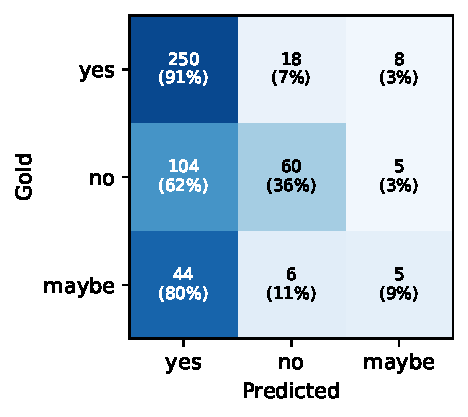
\includegraphics[width=0.42\linewidth]{figures/fig_baseline_confusion.pdf}
\hfill
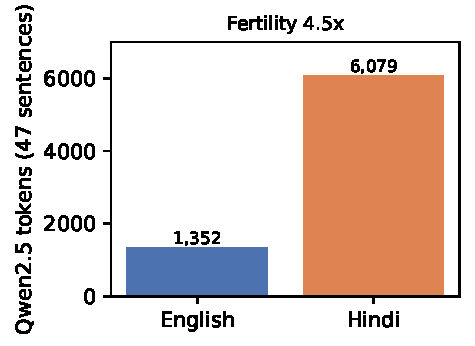
\includegraphics[width=0.40\linewidth]{figures/fig_pilot_tokens.pdf}
\caption{Left: confusion matrix of the English baseline on dev (rows: gold). Right: Qwen2.5 token counts for the same 47 sentences in English and in their Hindi translation (pilot).}
\label{fig:confusion}
\end{figure}

\subsection{Translation pilot (Hindi, 5 dev items)}
The pilot translated 47 sentences into Hindi with no truncation. Thirty-two were also back-translated before the run was stopped for time. All 34 numbers in the English source appear in the Hindi output after digit normalisation, and 20 of 20 survive the round trip. The same content costs Qwen2.5 6,079 tokens in Hindi versus 1,352 in English, a fertility of $4.5\times$ (Figure~\ref{fig:confusion}, right). We also found broken decimals in the source data (e.g., ``14. 1\%''), which the translator preserves. Five items is a pipeline check, not an estimate.

\subsection{Native vs Translate-Test (test set)}

\begin{table}[t]
\caption{Test-set results (n = 500, Qwen2.5-1.5B-Instruct, prompt P0). $\Delta$ = TT $-$ NATIVE macro-F1 with paired bootstrap 95\% CI (10,000 resamples); $p$ = Holm-adjusted exact McNemar; $\kappa$ = Cohen's kappa against the model's own EN predictions. Source: \texttt{results/tables/test/}.}
\label{tab:main}
\footnotesize
\setlength{\tabcolsep}{3.5pt}
\begin{tabular}{llcccccc}
\toprule
Language (tier) & Condition & Acc. & Macro-F1 & F1 yes/no/maybe & $\Delta$ [95\% CI] & $p$ & $\kappa$ vs EN \\
\midrule
--- & Majority & 55.20 & 23.71 & 71.1 / 0.0 / 0.0 & & & \\
English & EN & 63.60 & 44.59 & 75.4 / 47.4 / 11.0 & & & \\
\midrule
Hindi (mid) & NATIVE & 41.60 & 30.04 & 63.5 / \phantom{0}7.8 / 18.8 & \multirow{2}{*}{$+12.88$ [$+7.79$, $+17.87$]} & \multirow{2}{*}{$<10^{-15}$} & 0.16 \\
 & TT & 62.20 & 42.92 & 74.7 / 46.2 / \phantom{0}7.9 & & & 0.68 \\
\midrule
Odia (very low) & NATIVE & 47.60 & 28.86 & 65.2 / 17.4 / \phantom{0}4.1 & \multirow{2}{*}{$+12.42$ [$+7.09$, $+17.58$]} & \multirow{2}{*}{$1.4\times10^{-7}$} & 0.06 \\
 & TT & 60.40 & 41.28 & 72.7 / 45.8 / \phantom{0}5.4 & & & 0.58 \\
\bottomrule
\end{tabular}
\end{table}

\textbf{RQ1.} TT outperforms NATIVE significantly in both languages, and both pre-registered criteria agree (Table~\ref{tab:main}, Figure~\ref{fig:test}, left). Of the discordant items, TT alone is correct on 136 vs 33 (Hindi) and 106 vs 42 (Odia). H1 (TT $>$ NATIVE for Odia) is \textbf{supported}. H2 (NATIVE $\geq$ TT for Hindi) is \textbf{contradicted}: TT is significantly better for Hindi too. A paired bootstrap of the difference between the two gaps (added after peer review, so exploratory) gives $+0.46$ [$-5.01$, $+6.13$]. The gaps do not differ detectably, but tier differences of up to about 6 points cannot be ruled out. TT loses only 1.67 (Hindi) and 3.31 (Odia) macro-F1 relative to EN.

The per-class scores locate the failure. Under NATIVE the model nearly stops predicting ``no'': recall on gold ``no'' falls from 60/169 (EN) to 7/169 for Hindi and 21/169 for Odia. For Hindi, predictions move to ``maybe'' (211 of 500, vs 18 for EN); for Odia they move to ``yes'' (384). Both NATIVE conditions score \emph{below} the Majority baseline in accuracy (41.60 and 47.60 vs 55.20), although both remain above it in macro-F1.

\textbf{RQ2.} TT answers agree with the model's own English answers on 88.8\% (Hindi, $\kappa = 0.68$) and 84.8\% (Odia, $\kappa = 0.58$) of items. NATIVE agreement is 54.6\% ($\kappa = 0.16$) and 66.2\% ($\kappa = 0.06$). The higher raw agreement for Odia NATIVE reflects its shift toward ``yes'', the label EN predicts most, rather than consistency: its $\kappa$ is close to chance. Of the items EN answers correctly, NATIVE gets 42.8\% (Hindi) and 34.0\% (Odia) wrong; TT gets 8.2\% and 12.3\% wrong.

\textbf{RQ3.} Full prompts cost Qwen2.5 a mean $3.6\times$ (Hindi) and $7.8\times$ (Odia) the English token count. This is lower than the pilot's content-only $4.5\times$ for Hindi because the shared English instruction is included; median prompt length is 392 tokens in English, 1,417 in Hindi and 3,053 in Odia. Numbers survive EN$\to$X translation in 93.5\% (Hindi) and 81.5\% (Odia) of cases, and the full round trip in 90.4\% and 78.9\%; round-trip chrF is 80.6 and 69.2. H3 (lower number preservation for Odia) is \textbf{supported} descriptively; it was pre-registered without a significance test (Figure~\ref{fig:test}, right). The larger token cost for Odia does \emph{not} come with a larger NATIVE loss than Hindi, so fertility alone does not explain the native drop.

\begin{figure}[t]
\centering
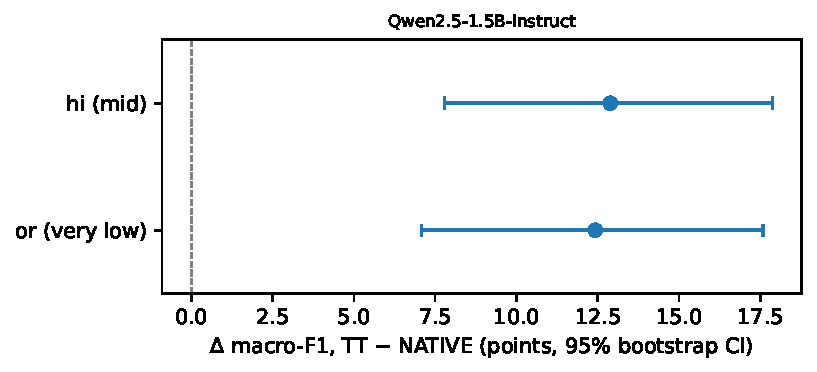
\includegraphics[width=0.52\linewidth]{figures/fig1_forest_tt_vs_native.pdf}
\hfill
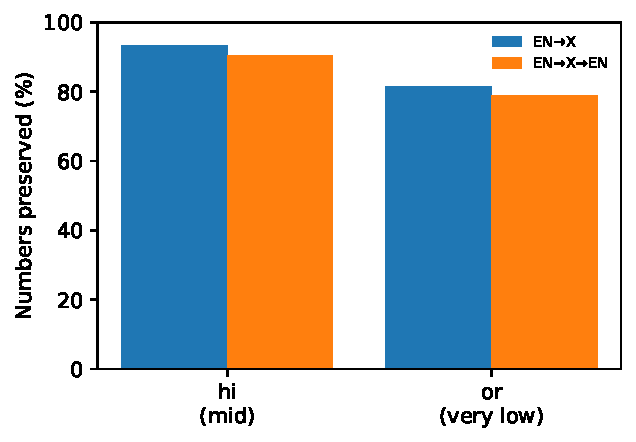
\includegraphics[width=0.44\linewidth]{figures/fig3_number_preservation.pdf}
\caption{Left: $\Delta$ macro-F1 (TT $-$ NATIVE) with paired bootstrap 95\% CI on the test set. Right: share of source numbers preserved after EN$\to$X translation and after the round trip.}
\label{fig:test}
\end{figure}

\subsection{Exploratory: translation degeneration in Odia (not pre-registered)}
In 506 of 5,285 unique Odia sentences (Hindi: 0), IndicTrans2 reached the 512-token limit without an end-of-sequence token. In 497 cases the output was a translation of plausible length followed by a long run of repeated full stops; the remaining 9 were repeated short fragments. No Odia reader has checked these outputs. Repeated runs (including shorter ones that ended normally) affect 398 of 500 Odia items, plus 3 with fragment repetition. Hindi is not free of the problem: 14 Hindi items contain shorter dot runs that ended before the limit, and none of these runs occurs in the English source. The back-translation inherits the runs. We added this analysis after seeing the test results, so it is exploratory. The primary result is unchanged. On the 99 Odia items with no flagged segment, $\Delta$ is $+13.02$ [$+2.50$, $+22.35$] (McNemar $p = 0.016$), similar to the 401 affected items ($+12.47$). Removing the repeated runs changes Odia token fertility by about 1\%. The degeneration therefore does not explain the TT advantage, but it is a quality defect that a real deployment would need to handle.

%% ===================================================================
\section{Discussion}

\textbf{Main finding.} Singh et al.~\cite{singh2025indicqa} found that TT helps very low-resource languages while native processing is competitive for mid-resource ones. In our scientific QA setting, with a 1.5B model, TT helps \emph{both} tiers, by amounts that do not differ detectably. The predicted tier difference does not appear, although our data cannot exclude a difference of a few points. We see three possible reasons, which we have not tested. (i) Model size: a 1.5B model may have too little Hindi competence for native processing to compete; we did not match the models evaluated in~\cite{singh2025indicqa}. (ii) Domain: biomedical terminology may be harder to understand in translated Hindi than general text. (iii) Input construction: our ``native'' text is machine-translated. It may contain translation artefacts that a model reads more easily once translated back into English. The size of the TT recovery (within 1.7--3.3 macro-F1 of EN) suggests that IndicTrans2 preserves most of the information the model needs. This is \emph{consistent with} the NATIVE failure lying in the model's comprehension of Indic-script input, but it does not rule out (iii).

\textbf{Why ``no'' disappears.} Under NATIVE, the model loses almost all recall on ``no''. It falls back to ``maybe'' (Hindi) or ``yes'' (Odia) instead. A plausible explanation is that answering ``no'' requires recognising a negative or null finding in the abstract, and this is exactly the information a model with weak target-language comprehension loses. ``Maybe'' and ``yes'' behave as default answers under uncertainty. We did not test this mechanism, and calibration could change the picture (Section~\ref{sec:limits}).

\textbf{Cost and numbers.} TT is also far cheaper at inference: the median Odia prompt is 3,053 tokens vs 424 for TT-Odia. Translation itself is not free (about 45 min of T4 time for Odia vs 16 min for Hindi). Odia loses more numbers (81.5\% vs 93.5\% preserved), consistent with~\cite{agrawal2024translation}. TT-Odia nevertheless stays within 3.3 macro-F1 of EN. We did not link number loss to answer changes item by item, so whether lost numbers matter for this task remains open; RQ3's ``relate to failures'' is answered only at the aggregate level.

\textbf{What is not claimed.} We do not claim that native processing is worse in general. That would need native-authored text, larger models and more than one language per tier. We do not claim causal mechanisms for the ``no'' collapse.

%% ===================================================================
\section{Limitations}
\label{sec:limits}
(1) A single 1.5B model: no cross-model check. (2) One language per resource tier, so tier and language effects cannot be separated. (3) ``Native'' inputs are machine-translated rather than authored natively~\cite{huang2025benchmax}. As a result, TT is a round trip of English text (round-trip chrF 80.6 and 69.2) and is close to EN by construction. With native-authored documents, TT would involve one translation step from human-written text, and its advantage could be smaller. (4) PubMedQA may be in the model's pretraining data; the paired design reduces but does not remove this concern. (5) Uncalibrated log-likelihood scoring with a strong yes-bias. (6) No prompt-sensitivity analysis. (7) Development runs and test runs used different hardware and transformers versions; this is documented, and all test conditions share one environment. Native conditions have more near-ties between the top two labels (margin $<0.05$ nats: 30 Hindi and 26 Odia items, vs 6--10 for EN and TT). Such items can flip across GPUs; one did when we re-scored it on Apple MPS. (8) IndicTrans2 degenerated on 9.6\% of Odia sentences (repeated full stops). The exploratory clean-subset analysis suggests this does not drive the result, but it rests on only 99 items.

%% ===================================================================
\section{Reproducibility and AI Use}
Code, the frozen protocols (v1--v4 with SHA-256 hashes), decision log, baseline-validation report and all genuine outputs are in the project repository. Commands are listed in its README.

This work used Claude Code (Anthropic) as a supervised assistant for literature verification, code generation, debugging and drafting. Every number in this paper comes from executed code or a cited source. The AI-assistance log records each significant AI proposal, how it was verified, and the human decision. It includes several AI errors that were caught: an unsupported language-tier assumption, a YAML syntax error, an evaluator bug, a download script that misreported success, a patch that silently changed the beam-search setting, a notebook whose non-blocking login made the first test run fail, and an unverified comparison with prior work that was removed before submission. An AI-written critical review (\texttt{docs/P16\_peer\_review.md}) also found a factual error in a draft of Section~5.5, which was corrected.

%% ===================================================================
\section{Conclusion}
We ran a pre-registered, validated comparison of native and Translate-Test processing for scientific QA in Hindi and Odia. On the PubMedQA test set, translating to English first improves a zero-shot Qwen2.5-1.5B model by about 12.5 macro-F1 points in \emph{both} languages and recovers nearly all of its English performance. Native input mainly destroys the model's ability to answer ``no''. The general-domain finding that native processing is competitive for mid-resource languages does not transfer to this setting. For this model and design, TT is the stronger and cheaper option. Whether this holds for native-authored scientific text and larger models is the clearest next question.

\bibliographystyle{ACM-Reference-Format}
\bibliography{references}

\end{document}
